\subsection{Testing for Weak SSL/TSL Ciphers, Insufficient Transport Layer Protection - OTG-CRYPST-001}
\paragraph{BANK-APP} \mbox{}
\begin{longtable*}{p{.20\textwidth} | p{.80\textwidth}}
	\hline
	& \textbf{BANK-APP} \\
	\hline
	\textbf{Observation} &
	It has been found that application works only on HTTP and does not support transmission over HTTPS. Neither does the application encrypt data used in requests. It is also observed that there are no ports having SSL services and hence no further testing could be done.
	\\\\
	\textbf{Discovery} &
	Steps:
	Tests to determine transmission over HTTP/HTTPS has been described in section \ref{OTG-AUTHN-001}.
	\underline{\textbf{Test for HTTP Basic Authentication: }}
	1. Open the Login page in the browser.
	2. Open Firebug in Firefox or Developer Tools in Chrome and navigate to the Network tab.
	3. Enter credentials in the login form and click on "Submit".
	4. Observe the request captured in the Network tab.
	5. The response does not contain the "WWW-Authenticate" header indicating that the server does not use Basic Authentication.
	\underline{\textbf{Test for SSL services: }}
	1. Open the terminal and type nmap -sV --reason -PN -n --top-ports 100 <IP-address>.
	2. To also check typical ports with SSL support, type nmap --script ssl-cert,ssl-enum-ciphers -p 443,465,993,995 <IP-address>. See Figure \ref{nmap_ssl_ports}.
	Observing the output, it can be concluded that none of the ports on the virtual machine support SSL service.
	\\\\
	\textbf{Impact} &
	NA
	\\\\
	\textbf{CVSS} &
	NA
	\\
	\hline
\end{longtable*}
\begin{figure}[ht]
	\centering
	\begin{subfigure}{.45\textwidth}
		\centering
		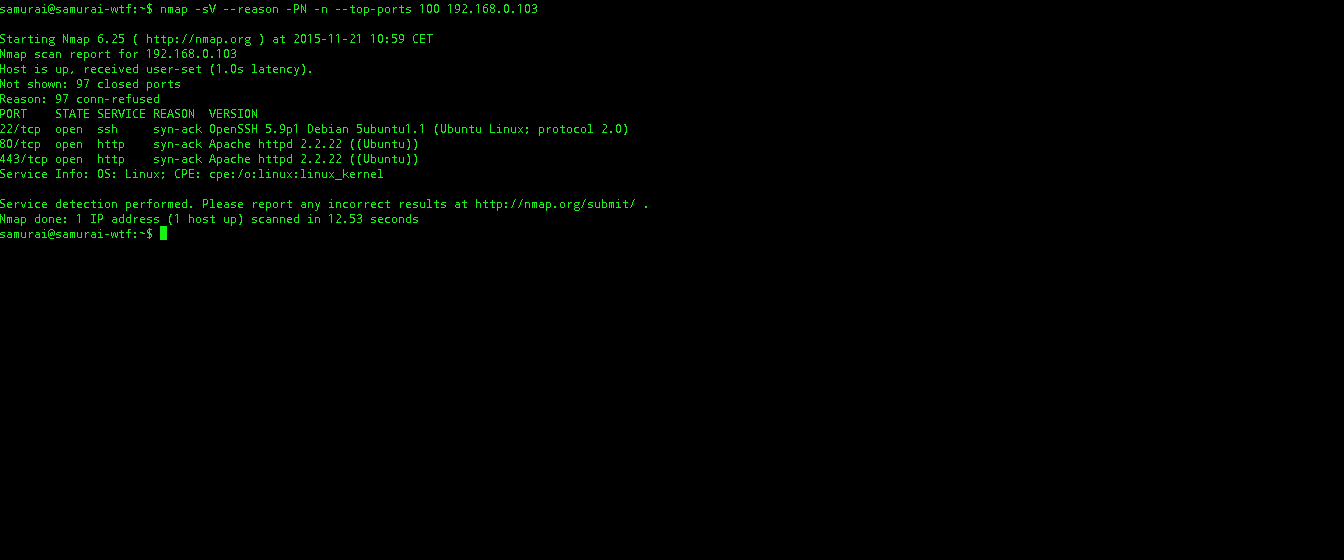
\includegraphics[width=.9\linewidth]{figures/OTG-CRYPST-001_1.png}
		\caption{Nmap - Generic check for ports with SSL support}
	\end{subfigure}\hfill%
	\begin{subfigure}{.45\textwidth}
		\centering
		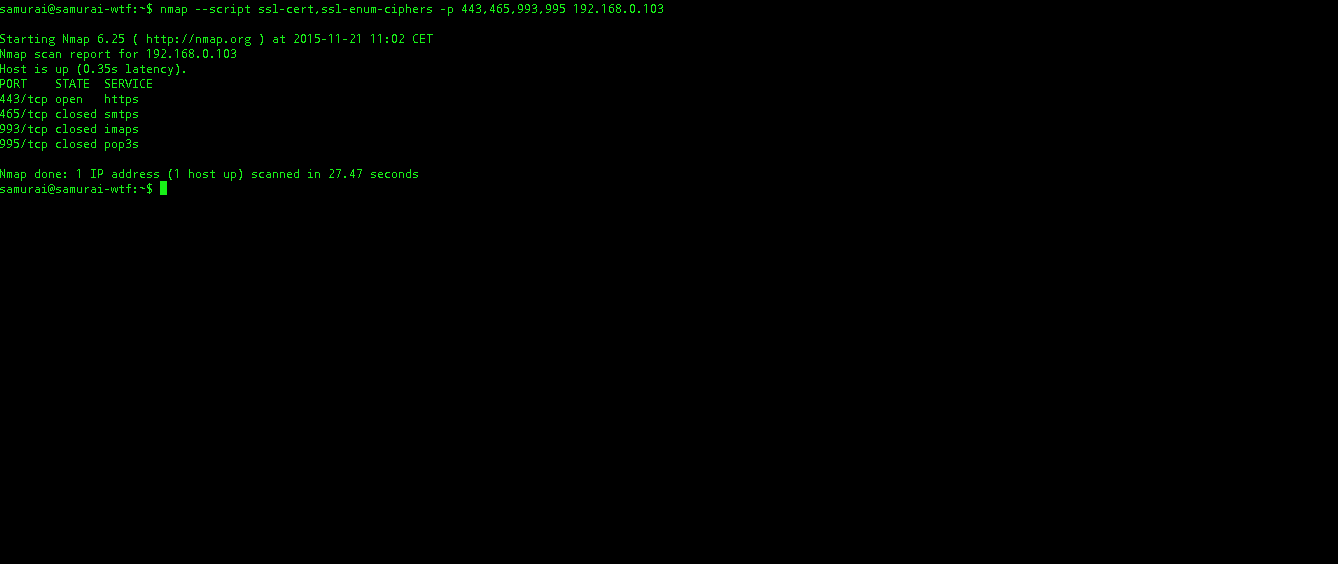
\includegraphics[width=.9\linewidth]{figures/OTG-CRYPST-001_2.png}
		\caption{Nmap - Check for typical ports with SSL configuration}
	\end{subfigure}
	\caption{Testing for ports with SSL configuration}
	\label{fig:nmap_ssl_ports}
\end{figure}

\paragraph{SecureBank} \mbox{}
\begin{longtable*}{p{.20\textwidth} | p{.80\textwidth}}
	\hline
	& \textbf{SecureBank} \\
	\hline
	\textbf{Observation} &
	It has been found that application works only on HTTP and does not support transmission over HTTPS. Neither does the application encrypt data used in requests. It is also observed that there are no ports having SSL services and hence no further testing could be done.
	\\\\
	\textbf{Discovery} &
	Same as observed for BANK-APP.
	\\\\
	\textbf{Likelihood} &
	NA
	\\\\
	\textbf{Impact} &
	NA
	\\\\
	\textbf{CVSS} &
	NA
	\\
	\hline
\end{longtable*}
\clearpage